\documentclass{article}
\usepackage{graphicx}
\graphicspath{ {./} }
\usepackage{color}

\usepackage{amsmath}
\usepackage{commath}
\usepackage{amssymb}
\usepackage{listings}
\usepackage{algorithm2e}
\usepackage{float}

\usepackage{hyperref}
\hypersetup{linktoc=all}

\usepackage{listings}
\usepackage{geometry}
\geometry{margin=1in}
\usepackage{color}
\definecolor{light-gray}{gray}{0.95}
\lstset{numbers=right,
                basicstyle=\small,
                numberstyle=\tiny,
                breaklines=true,
                backgroundcolor=\color{light-gray},
                numbersep=5pt,
                xleftmargin=.5in,
                xrightmargin=.5in}

\sloppy
\definecolor{lightgray}{gray}{0.5}
\setlength{\parindent}{0pt}

\begin{document}

\title{Lab 6: Contrast Enhancement and Resampling}
\author{Brian Hosler \& Sarah Peachey }
\maketitle

\qquad Image editing operations which are intended to only
increase the perceptual quality of images, or not change the
content, leave traces or fingerprints, which can be found by
looking at statistics of the image. For example, contrast
enhancement can be found by looking at pixel value histograms.
Resampling can be detected using generic prediction error
filters, and analysing the frequency of the estimated
probability of errors.

\tableofcontents
\newpage



\section{Detecting Image Contrast Enhancement}

\qquad Contrast enhancement through gamma correction is a
deterministic, non-linear mapping of pixel values. This
non-linearity causes multiple pixel values to map to the
same pixel value, and consecutive pixel values to be mapped
further apart. Both of these phenomina are visible in the
pixel value histograms of contrast enhanced images. The
pixel value histograms of four images were viewed using
MATLAB to determine if they were contrast enhanced or not.
Next, several images were enhanced using gamma correction
with gamma below and above 1, to view the effects that
different gamma have on the histograms.

\begin{lstlisting}
ce1=imread('Assignment6Files/imageCE1.tif');
ce2=imread('Assignment6Files/imageCE2.tif');
ce3=imread('Assignment6Files/imageCE3.tif');
ce4=imread('Assignment6Files/imageCE4.tif');
ce5=imread('Assignment6Files/imageCE5.tif');

subplot(1,2,1)
imhist(ce1)%ENHANCED
subplot(1,2,2)
imhist(ce2)
figure
subplot(1,2,1)
imhist(ce3)%ENHANCED
subplot(1,2,2)
imhist(ce4)

ui1=imread('Assignment6Files/unaltIm1.tif');
ui2=imread('Assignment6Files/unaltIm2.tif');
ui3=imread('Assignment6Files/unaltIm3.tif');

figure
subplot(3,1,1)
imhist(Gcorrection(ui1,.7))
subplot(3,1,2)
imhist(ui1)
subplot(3,1,3)
imhist(Gcorrection(ui1,1.3))

figure
subplot(3,1,1)
imhist(Gcorrection(ui2,.7))
subplot(3,1,2)
imhist(ui2)
subplot(3,1,3)
imhist(Gcorrection(ui2,1.3))

figure
subplot(3,1,1)
imhist(Gcorrection(ui3,.7))
subplot(3,1,2)
imhist(ui3)
subplot(3,1,3)
imhist(Gcorrection(ui3,1.3))

figure
imhist(ce5)

type('Gcorrection.m')
\end{lstlisting}

\newpage
\begin{lstlisting}
function [ img_out ] = Gcorrection(img_in, gama)
%Does gamma correction using the equation:
%   new=2558(old/255)^gamma
    img_out=uint8(255*(double(img_in)/255).^gama);
end

\end{lstlisting}
    
\qquad Given the histograms of images 1-4, we found the images
1 and 3 show contrast enhancement fingerprints, where images
2 and 4 have smoother histograms that do not appear to be
altered. The sudden peaks and gaps in the histogram are
characteristic of contrast enhanced images.

\qquad A number less than one raised to a power greater than one will
result in a number even less than the original. Rounding will
cause smaller numbers to be mapped together, while larger
numbers will be mapped apart. Gamma correction with gamma greater
than 1 will result in locally expansive regions in the area of the
histogram representing light pixels. This will correspond
to locally contractive regions in the area of the histogram
representing dark pixel values.
Gamma values less than 1 will cause the opposite behavior,
locally expansive regions on the left of the histogram, and
contractive regions on the right.
Given this, it is likely that imageCE5.tif underwent gamma
correction where gamma was less than 1.

\begin{figure}[H]
\centering
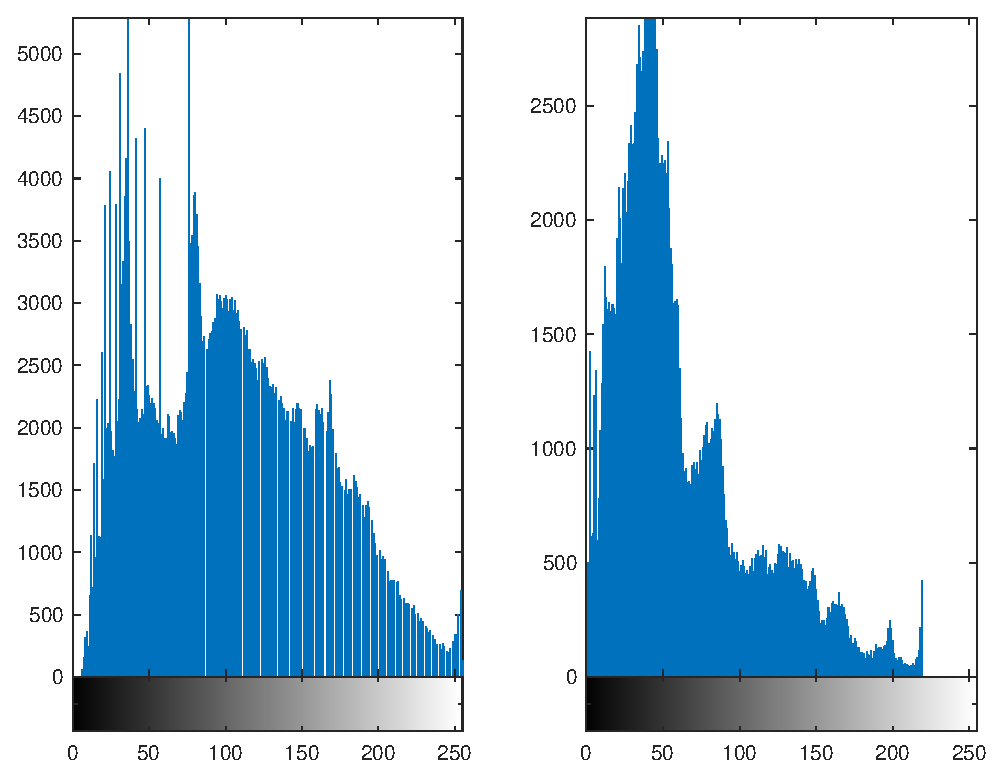
\includegraphics [width=5in,height=3in]{lab6_01.eps}
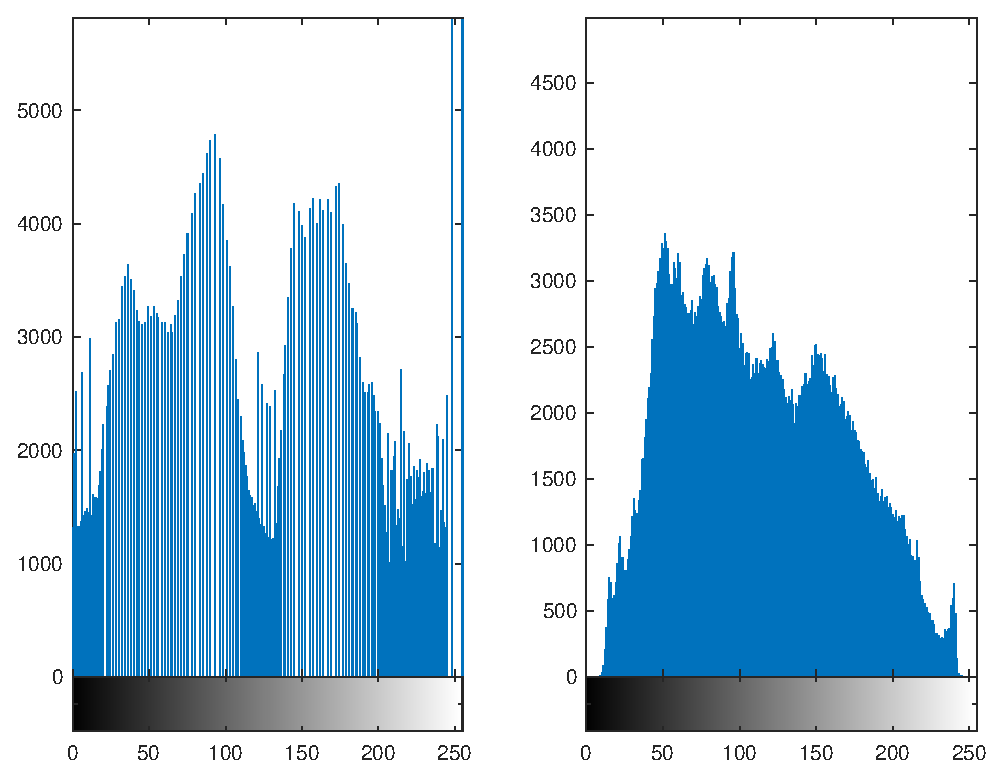
\includegraphics [width=5in,height=3in]{lab6_02.eps}
\caption{Pixel value histograms of imagesCE1.tif, imageCE2.tif,
imageCE3.tif and imageCE4.tif}
\end{figure}


\begin{figure}[H]
\centering
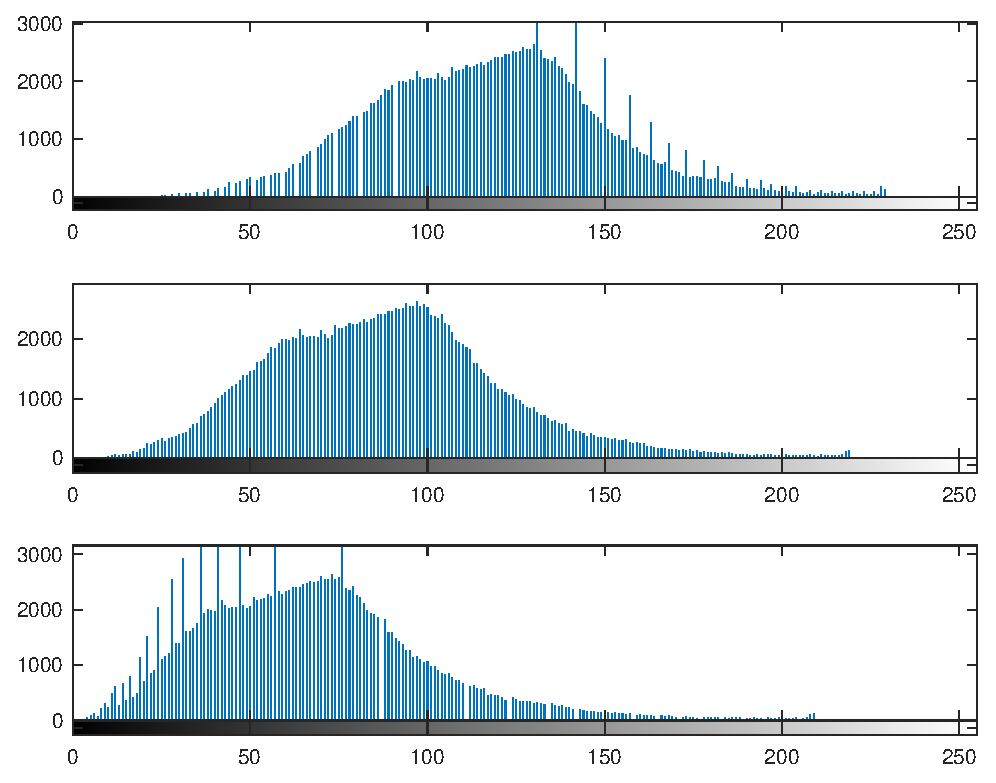
\includegraphics [width=4in]{lab6_03.eps}
\caption{Pixel value histograms of unaltIm1.tif after gamma correction
of 0.7, 1(no correction), and 1.3}
\end{figure}

\begin{figure}[H]
\centering
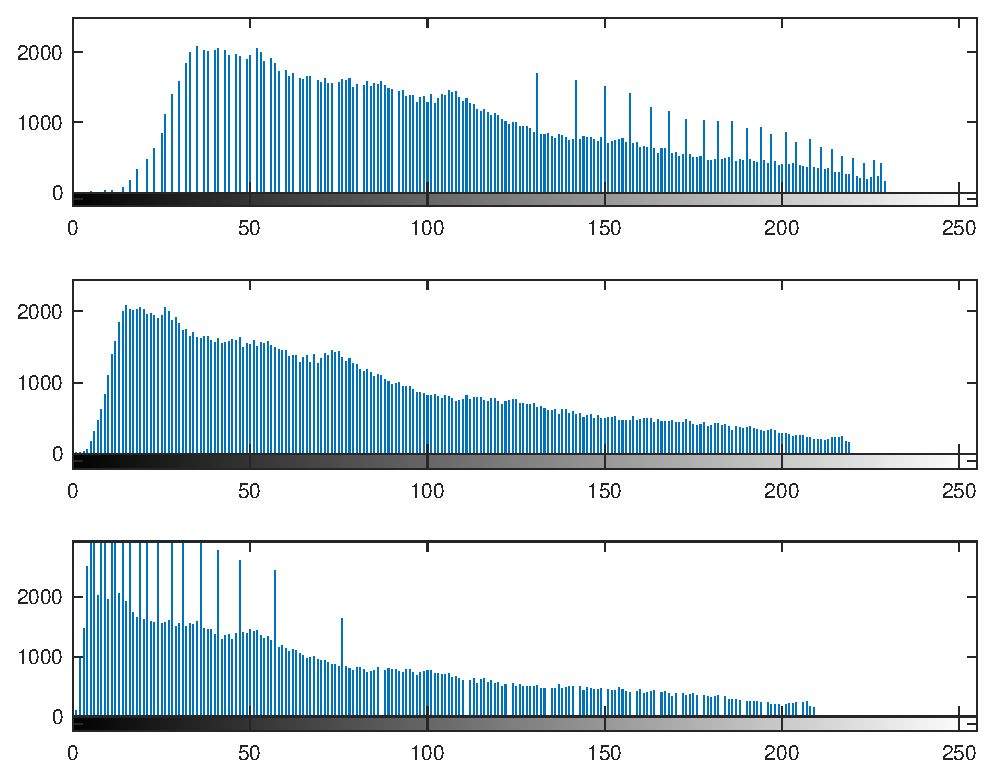
\includegraphics [width=4in]{lab6_04.eps}
\caption{Pixel value histograms of unaltIm2.tif after gamma correction
of 0.7, 1(no correction), and 1.3}
\end{figure}

\begin{figure}[H]
\centering
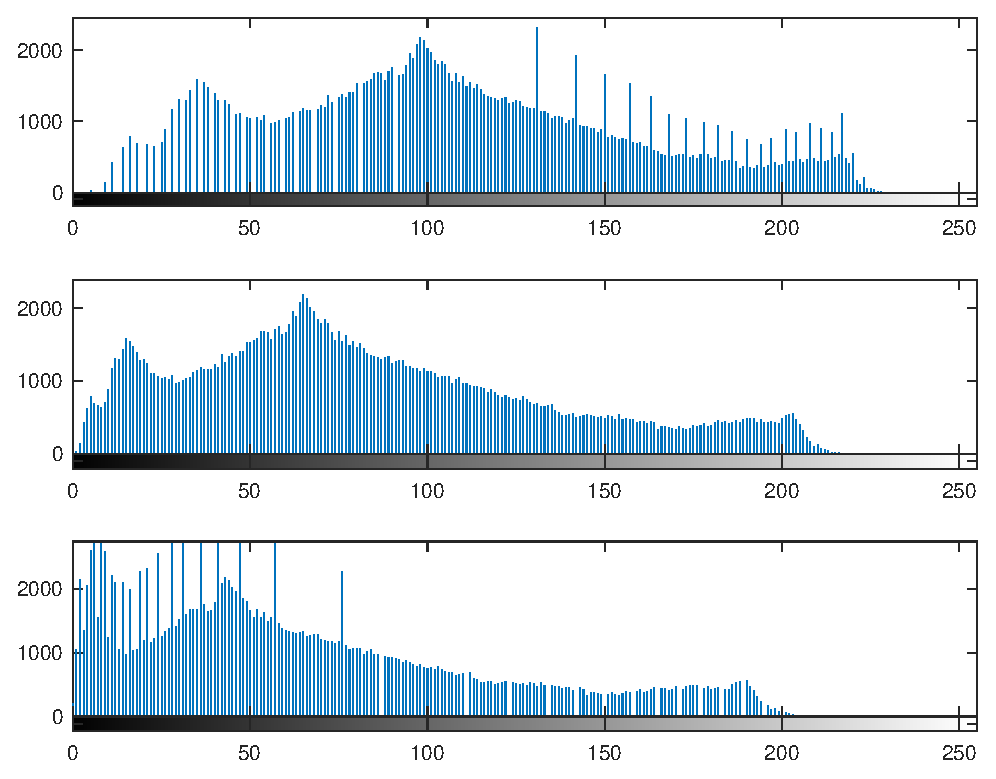
\includegraphics [width=4in]{lab6_05.eps}
\caption{Pixel value histograms of unaltIm3.tif after gamma correction
of 0.7, 1(no correction), and 1.3}
\end{figure}

\begin{figure}[H]
\centering
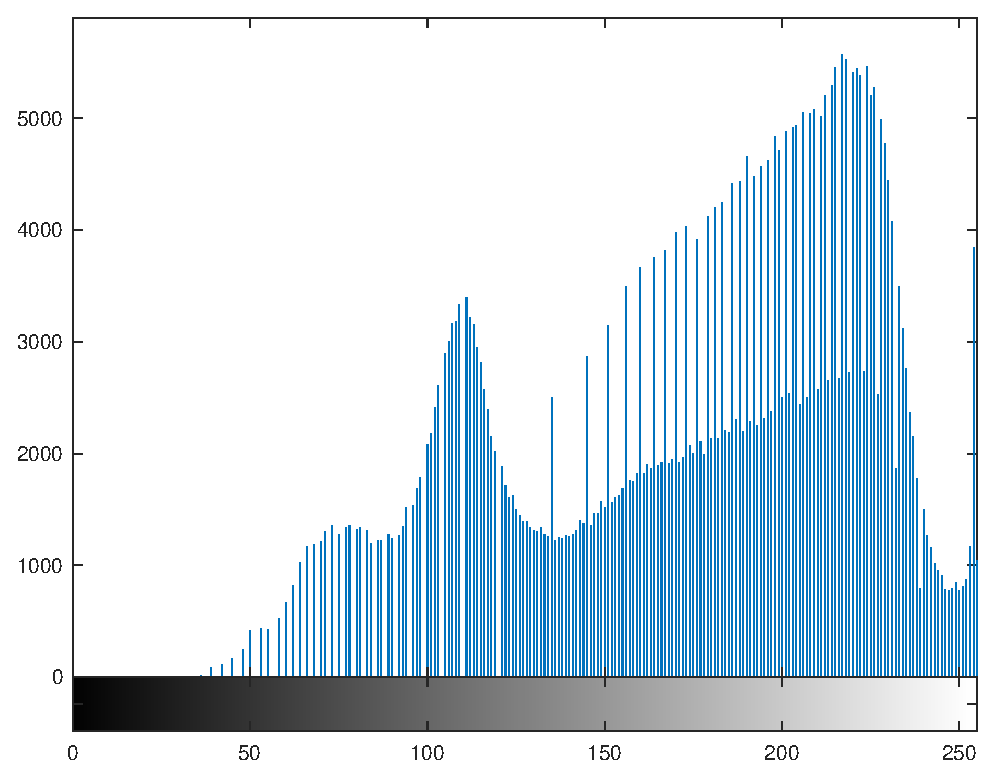
\includegraphics [width=4in]{lab6_06.eps}
\caption{Pixel value histogram of imageCE5.tif showing gamma correction
where gamma os less than 1}
\end{figure}


\section{Detecting Image Resampling and Resizing}

\qquad One of the most common image resampling operations is resizing. Image
resampling fingerprints can be detected with the Popescu and Faird method
but is computationally complex. The algorithm derived by Kirchner is an
approximation of the same results but far less computationally intense. 
Kirchner's algorithm uses a fixed linear filter to approximate relationships
between pixel values. The variance resulting from the predicted pixel error
will be periodic. As seen in the below function Kirchner's algorithm, the
image is first filtered with the linear prediction filter, then the error is
calculated, and the p-map is then approximated with the below equation. 
 
\begin{align} 
	p(x,y)=\lambda exp^{\frac{-e(x,y)^\tau}{\sigma}}
\end{align}



\begin{lstlisting}
function [ pmap_approx ] = kirchners( im )
%KIRCHNERS  approximates the pmap 
%   Detailed explanation goes here
I=double(im); 
% 1)
alpha=[-0.25 0.5 -0.25; 0.5 0 0.5;-0.25 0.5 -.25]; 
I_hat=filter2(alpha, I); 
% 2)
pred_error=I-I_hat; 
% 3)
lambda=1; 
tau=2; 
sigma=1; 
pmap_approx=lambda*exp((-pred_error.^tau)./sigma); 
end
\end{lstlisting} 

\begin{lstlisting}
im1=imread('Assignment6Files/resamp1.tif');
im2=imread('Assignment6Files/resamp2.tif');
im3=imread('Assignment6Files/resamp3.tif');
im4=imread('Assignment6Files/resamp4.tif');
p1= kirchners( im1 );
p2= kirchners( im2 );
p3= kirchners( im3 );
p4= kirchners( im4 );

figure
subplot(2,2,1)
imagesc(p1)
colormap(cool)
subplot(2,2,2)
imagesc(p2)
subplot(2,2,3)
imagesc(p3)
subplot(2,2,4)
imagesc(p4)

figure
subplot(2,2,1)
showFreqPmap(p1)
subplot(2,2,2)
showFreqPmap(p2)
subplot(2,2,3)
showFreqPmap(p3)
subplot(2,2,4)
showFreqPmap(p4)
type('kirchners.m')
\end{lstlisting}
    

Below shows the p-map for the several images, the top-right and bottom-left
images appear to have a periodic grid, so they are clearly resized. So just
based off the p-maps resampIm2.tif and resampIm3.tif appear to be resized
but the other two do not. But then the frequency of the p-map is
calculated and also shown below, 
which showed that the not only 2 and 3 but also resampIm4.tif was resampled
in at least one direction. 


\includegraphics [width=4in]{lab6_07.eps}

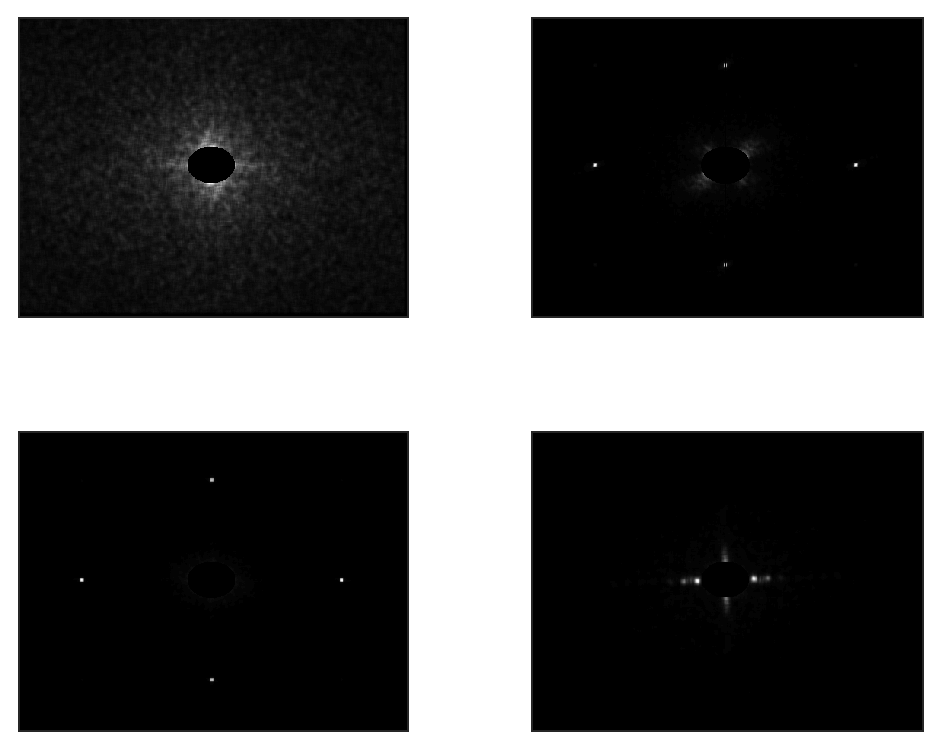
\includegraphics [width=4in]{lab6_08.eps}



\end{document}
    
